\subsection{模型假设}

出于精准针对用户推送的考虑,本文认为买方所能提供的销售记录是个体用户对商品的购买记录,
其中用户的个人的关键信息被隐去,只保留能刻画用户分类特征的一些信息,如性别、年龄和职业信息等。

针对第一题中买方对广告特征的评估存在随意性和主观性的问题,本题中不再需要买方对广告
进行参数化的评价,而只需提供广告类别和广告描述,卖方需要从这两个信息中提炼出广告的特征。

\begin{enumerate}[(1)]
    \item 假设买方在播视频广告的产品都是通过电视广告进行推销的,其它推销方式的影响忽略不计;
    \item 假设买方能准确记录下产品顾客的性别、年龄和职业信息;
    \item 假设买方给电视台提供的销售记录数据服从一定的分布性,能反应其各自受众之间的差异;
    \item 假设买方提供的广告类别准确,且提供的广告描述包含尽量多的关键词信息(包括商品类型、生产商、商品名等)
\end{enumerate}

\subsection{模型建立}

为建立面向已知销售和收视情况的推荐机制,本文提出一种基于深度学习的协同过滤模型。本文使用协同过滤(CollaboratIve Filtering)算法,先计算广告之间的相似度,找到与当前
广告相似的历史广告的销售记录和收看记录,再将这个广告推介给同一用户群体。

协同过滤算法在实际的推荐系统中有着广泛的应用,但在我们的推荐系统中,打分(Rating)矩阵仅由销售和收视情况来决定,则必然会产生打分矩阵稀疏的问题,从而导致推荐效果不理想。
因此,在我们的算法中,加入了深度学习模型和矩阵分解模型,能够从外部辅助信息和传统的打分信息中学习到更为有效地特征表示。

具体的深度学习的模型设计图如下:

\begin{figure}[H]
    \centering
    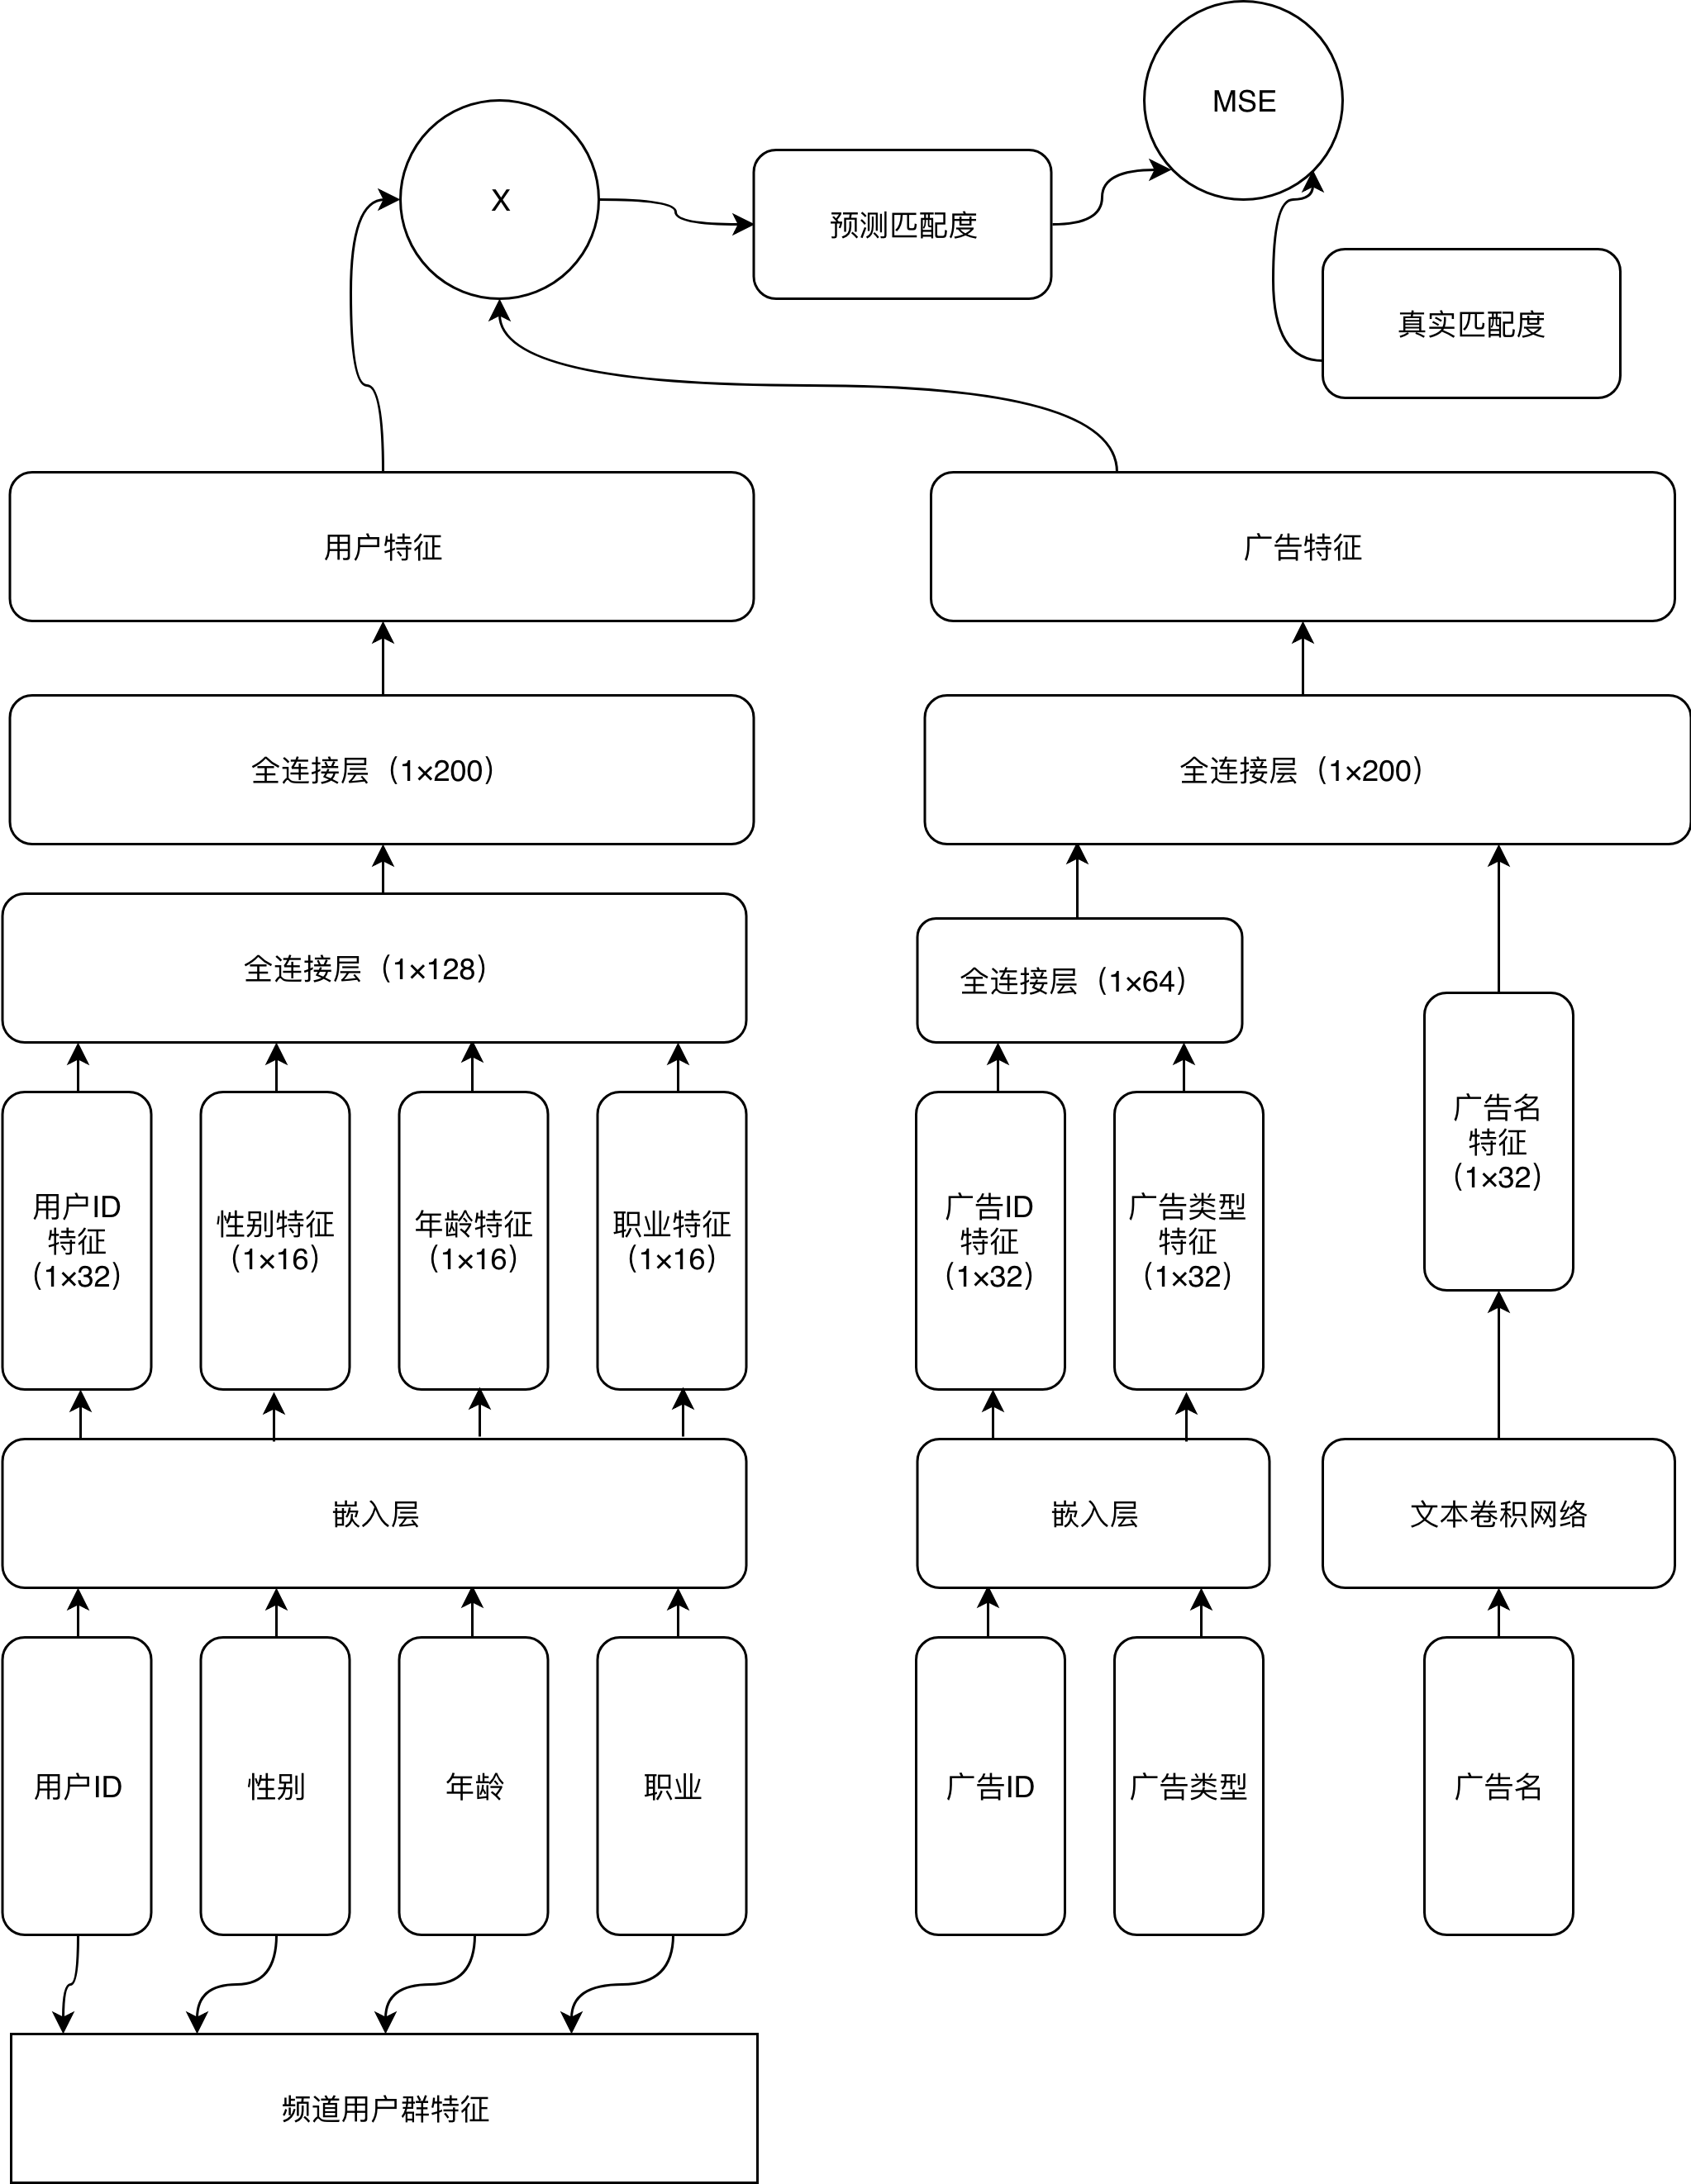
\includegraphics[scale=0.18]
        {resources/Advertisement.png}
    \caption{模型设计}
\end{figure}

\subsubsection{向量化操作}

\begin{enumerate}[(1)]
    \item 首先对数据集进行预处理操作,根据假设,用户数据集中包含了用户的ID、性别、年龄、职业信息,广告数据集中包含了广告类型的信息,为了便于处理,应将这些信息进行数值化处理,其对应关系如下:
    \begin{table}[H]
        \caption{用户年龄性别数值对应表}
        \begin{subtable}[H]{0.5\textwidth}
            \centering
            \caption{用户年龄数值对应表}
            \begin{tabular}{cccc}
            \Xhline{1.2pt}
            0        & 1     & 2     & 3     \\
            \hline
            Under 18 & 18-24 & 25-34 & 35-44 \\
            \Xhline{1.2pt}
            4        & 5     & 6     &       \\
            \hline
            45-49    & 50-55 & 56+   &      \\
            \Xhline{1.2pt}
            \end{tabular}
        \end{subtable}
        \begin{subtable}[H]{0.4\textwidth}
            \centering
            \caption{用户性别数值对应表}
            \begin{tabular}{cc}
            \Xhline{1.2pt}
            0 & 1 \\
            \hline
            女 & 男 \\
            \Xhline{1.2pt}
            \end{tabular}
        \end{subtable}
    \end{table}

    \begin{table}[H]
        \centering
        \caption{用户职业数值对应表}
        \begin{tabular}{cccc}
        \Xhline{1.2pt}
        0                     & 1                   & 2                    & 3                     \\
        \hline
        academic/educator     & artist              & clerical/admin       & college/grad student" \\
        \Xhline{1.2pt}
        4                     & 5                   & 6                    & 7                     \\
        \hline
        customer service      & doctor/health care  & executive/managerial & farmer                \\
        \Xhline{1.2pt}
        8                     & 9                   & 10                   & 11                    \\
        \hline
        homemaker             & K-12 student        & lawyer               & programmer            \\
        \Xhline{1.2pt}
        12                    & 13                  & 14                   & 15                    \\
        \hline
        retired               & sales/marketing     & scientist            & self-employed         \\
        \Xhline{1.2pt}
        16                    & 17                  & 18                   & 19                    \\
        \hline
        technician/engineer   & tradesman/craftsman & unemployed           & writer               \\
        \Xhline{1.2pt}
        \end{tabular}
    \end{table}
    \begin{table}[H]
        \centering
        \caption{广告类型数值对应表}
        \begin{tabular}{ccccc}
        \Xhline{1.2pt}
        0                            & 1                & 2                  & 3              & 4             \\
        \hline
        Life-style                   & Advertising-song & Purchase-reason    & Intuitive      & Visual-effect \\
        \Xhline{1.2pt}
        5                            & 6                & 7                  & 8              & 9             \\
        \hline
        Emotional                    & Humor            & Customer-recommend & Story          & Pleasant      \\
        \Xhline{1.2pt}
        10                           & 11               & 12                 & 13             & 14            \\
        \hline
        Passionate                   & Cartoon          & Rational           & Leben-passiert & Persuasive    \\
        \Xhline{1.2pt}
        15                           & 16               & 17                 & 18             &               \\
        \hline
        \textless{}PAD\textgreater{} & Demonstration    & Single-speaker     & Film           &              \\
        \Xhline{1.2pt}
        \end{tabular}
    \end{table}
    \item 接着用这些数字当做嵌入矩阵的索引,在网络的第一层使用了嵌入层,其维度是($N$,32)和($N$,16);
    \item 针对广告描述这段文本内容,本文采用了文本卷积网络的方式进行处理。
    先由每一个单词的嵌入向量组成的嵌入矩阵,然后接下来下一层使用多个不同尺寸(窗口大小)
    的卷积核在嵌入矩阵上做卷积,窗口大小指的是每次卷积覆盖几个单词。最后得到一个长向量,
    使用dropout做正则化,最终得到广告描述的向量;
    \item 从嵌入层索引出特征以后,将各特征传入全连接层,将输出再次传入全连接层,最终分别得到(1,200)的用户特征和广告特征两个特征向量。
\end{enumerate}

\subsubsection{训练网络}

本文在训练网络层次参考借鉴了Collective Matrix Factorization模型\citep{Singh}。

\begin{figure}[H]
    \centering
    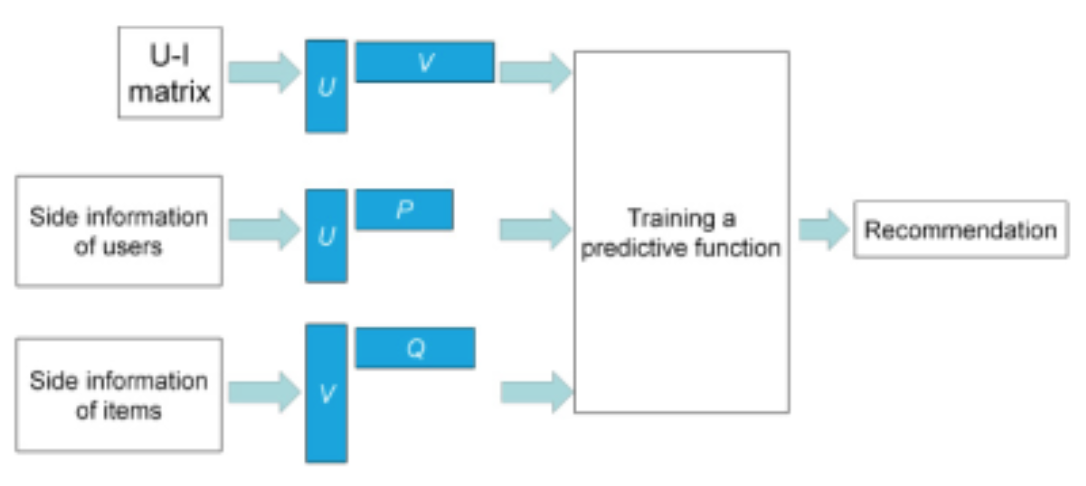
\includegraphics[scale=0.75]{cmf.png}
    \caption{Collective Matrix Factorization}
\end{figure}

这里CMF模型通过分别分解打分矩阵$\matr{R}$,用户、广告的辅助信息矩阵,
其中用户和广告出现在多个矩阵中,其所分解的隐向量都是一致的、共享的,从而建立联系。

在上述深度学习的模型的具体实现中,本文使用了激活函数ReLu来实现模型的优化:
\begin{equation}
    f(x)=\max(0,x)
\end{equation}

\begin{figure}[H]
    \centering
    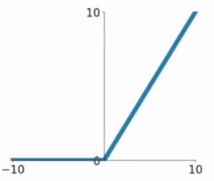
\includegraphics[scale=0.8]{ReLu.png}
    \caption{ReLu激活函数}
\end{figure}

其对于模型的优化在于:
\begin{itemize}
    \item 在输入为正数的时候,不存在梯度饱和问题;
    \item 计算速度有较大提升。ReLU函数只有线性关系,因此不管是前向传播还是反向传播,
    都会比sigmod函数和tanh函数要快很多。因为sigmod函数和tanh函数都需要计算指数,
    所以计算速度会比较慢。
\end{itemize}
当然,经过测试,我们也发现了一些缺点:
\begin{itemize}
    \item 当输入是负数的时候,ReLU是完全不被激活的,这就表明一旦输入到了负数,
    ReLU就会失效。这样在前向传播过程中,问题还没有显露,有的区域是敏感的,
    有的是不敏感的。但是到了反向传播过程中,输入负数,梯度就会完全降到0,
    这个和sigmod函数、tanh函数有一样的问题。
    \item ReLU函数的输出要么是0,要么是正数,这也就是说,
    ReLU函数不是以0为中心的函数。
\end{itemize}

\subsubsection{预测与推荐}

在协同过滤算法中,将特定的广告推送给用户的实质就是预测用户对该广告的评分,并将
对其评分最高的$N$个用户作为推送的对象。

\begin{itemize}
    \item 给定打分矩阵$ \matr{R}\in \BR^{m\times n}$,用户和广告的辅助信息分别是
    $ X\in \BR^{m\times p}$ 和 $Y\in \BR^{n\times q}$;
    \item $u_i,v_j \in \BR^{k}$ 分别表示分别表示第$i$个用户和第$j$个广告的隐含特征向量,
    k 表示维度,那么$ U=u_{1:m},V=v_{i:n}$ 就是我们学习的目标———用户和广告的隐含表示,
    进而预测用户对广告的打分;
    \item 从矩阵分解的角度来说,就是求解
    \begin{equation}
        \arg \min_{U,V} \mathcal{L}(R,UV^{\top})+\lambda(\abs{U}_F^2+\abs{V}_F^2)
    \end{equation}
    的过程。
\end{itemize}

在这里本文将基于用户的协同过滤算法与基于广告的协同过滤算法相结合,在上面方法实现的基础上寻求另一种求解的可能。

假设需要预测用户$A$对广告$M$的评分,首先对于广告$M$,根据训练数据集找出通过广告$M$购买商品的用户,
然后计算$A$和这些用户之间的相似度,依据相似度和这些用户对$M$的购买倾向,来预测用户$A$对广告$M$的评分。

在模型求解的过程中,我们发现根据训练数据集找出已经通过该电视广告购买商品的用户较容易,
预测结果的优劣关键在于如何计算用户$A$和这些
用户之间的相似度,以及采用何种方式来利用相似度和评分预测出用户$A$对广告$M$的购买倾向。其具体计算过程如下:

\begin{itemize}
    \item 首先,对于待预测的用户-广告(User::Advertisement)对,找出对于该广告已有购买记录的用户群Users[s];
    \item 然后,计算该用户与这些用户的余弦相似度$sim(u,i)$
    \begin{equation}
        sim(u,i)=\cos\theta=\frac{\sum\limits_{t=1}^{n}(u_t\times a_t)}{\sqrt{\sum\limits_{t=1}^{n}u_t^2}\times \sqrt{\sum\limits_{t=1}^{n}a_t^2}}
    \end{equation}
    \item 最后,利用
    \begin{equation}
        prescore(u,m)=\frac{\sum\limits_{i\in Users[s]}(sim(u,i)\times score(i,m))}{\sum\limits_{i\in Users[s]}sim(u,i)}
    \end{equation}
    预测用户$u$对广告$m$的购买倾向。
\end{itemize}

\subsection{模型求解}

由于本模型的求解需要大量的数据,而我们难以在互联网中找到类似的资源,因此本文
采用了推荐算法常用的开源数据集MovieLens数据集。
该数据集包含多个用户对多部电影的评级数据,也包括电影元数据信息和用户属性信息。
本文在引入该数据集时对该数据集做了一定的改动:
\begin{enumerate}
    \item 删除了一些不需要用户和物品的信息;
    \item 将原数据集中的电影名属性替换成了广告描述。
\end{enumerate}

本文的验证过程在Jupyter Notebook环境下。受制于正文篇幅限制,本文将代码和运行结果放在附录中。
此处只展示训练模型的均方差(MSE)结果:

\begin{figure}[H]
    \centering
    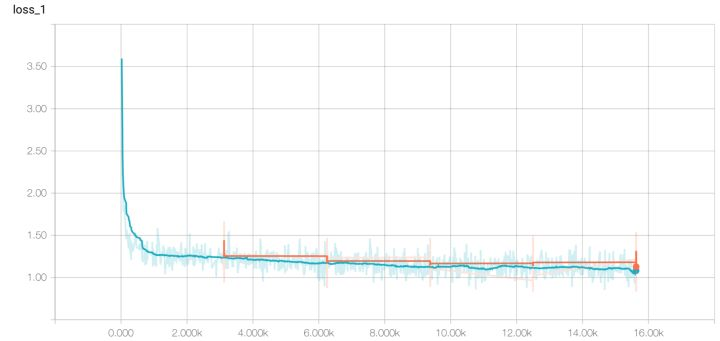
\includegraphics[scale=0.5]{TensorBoard.jpg}
    \caption{TensorBoard可视化结果}
\end{figure}

\subsection{模型评价}

经分析,本模型的优点如下:
\begin{itemize}
    \item 融合了外部辅助信息,学习的用户、广告表示较为丰满;
    \item 融合了历史数据,可以实时更新模型,从而动态地产生推荐;
    \item 虽模型训练时间花费较大,但模型训练后产生推荐相应速度很快。
\end{itemize}

本模型的缺点有:

\begin{itemize}
    \item 本模型采用的CMF方法中,特征的融合方式是直接将各向量首尾相连,这种融合过于简单直白,学习到的用户和广告的隐藏向量表示存在缺陷。
\end{itemize}
